\section{Introduction}
3D printing enables the fabrication of complex geometry under few design constraints compared to conventional fabrication techniques.
Recent developments have seen a rapid growth in both the use and capabilities of desktop 3D printing systems.
%The rapid spread of 3D printing through different industries and types of application calls for the possibility to manufacture a wide range of geometries while guaranteeing mechanical properties of the resulting parts.
Fused Deposition Modeling (FDM) is one of the most common 3D printing techniques.
It is widely used because of the versatility in the types of plastics which can be used and the relatively low running costs.
FDM printers are used, for example, in showcasing scale models of buildings, casings for electronics, prototypes blowmold parts, jigs and fixtures.
Recent research developments have investigated manufacturing complex volumetric structures such as microstructures~\cite{}, topology optimized structures~\cite{} and infill structures~\cite{}.
Many of these applications require 3D models with detailed features within the order of magnitude of the printing resolution, which restrains the field of the process planning algorithms.

FDM printers extrude semi-continuous beads of molten plastic through a nozzle, which moves along a planned toolpath within each layer of a 3D object.
Because the resolution of the positioning system is order of magnitude smaller than the width of the nozzle (typically from $??$ to $??$),
the toolpaths for filling the arbitrary polygonal shape of a layer with extrusion beads are following the contour of that layer.
\jun{I had difficulty to follow the logic behind this sentence}

The naive method for generating the shape filling toolpaths of a layer consists in performing inward offsets with the radius of the the nozzle from the outline shape.
However, for geometrical features which are not an exact multiple of the nozzle size this method produces areas where an extrusion bead is placed twice: \emph{overfill} areas; and other areas which are not filled at all: \emph{underfll} areas.
See \cref{intro_wedge}(top).
Overfills cause a buildup of pressure in the mechanical extrusion system, which can result in bulges or even a full print failure.
Underfills on the other hand, can cause a drastic decrease in the part stiffness or even for small features not to be printed at all.
These problems are exacerbated for models with layer outlines with small features, because the over- and underfill areas are large compared to the whole part.
In order to avoid over- and underfills in regions which are not as wide as an exact multiple of the nozzle size we need algorithms which produce toolpaths which employ adaptive bead width.
Some such toolpath generation techniques have already been developed.

\begin{figure}\centering
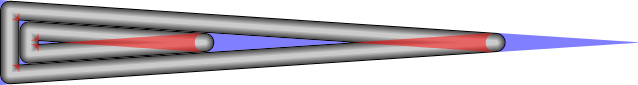
\includegraphics[width=\columnwidth]{sources/intro/TEST_naive_pretty.png}
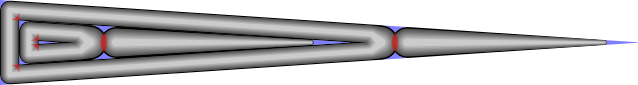
\includegraphics[width=\columnwidth]{sources/intro/TEST_Center_pretty.png}
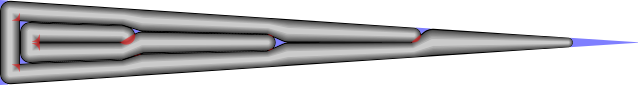
\includegraphics[width=\columnwidth]{sources/intro/TEST_Distributed_pretty.png}
\caption{
Toolpaths for a wedge shape using the naive offsetting approach (top), the approach by \citeauthor{Jin2017JMS}(middle) and our approach (bottom).
Red signifies overfill and blue underfill.
}
\label{intro_wedge}
\end{figure}



There is a large body of literature on relating process parameters such as bead width to various mechanical properties of the end part.
The bead width has been associated with total print time, the roughness of top surfaces, printing resolution and the strength of a part, through the contact area it makes with neighboring beads. \cite{N.Turner2014,ahn2002anisotropic}
In order to accurately fabricate a part restricted to prescribed mechanical properties, we need to generate toolpaths using the corresponding process parameters as close as possible.
We therefore develop a parametric system which can be used to generate toolpaths which not only avoid over- and underfill, but also keep the bead width closer to the nominal bead width compared to existing techniques.
See \cref{intro_wedge}(bottom).

%\subsection{Contributions}
A polygonal shape with a width of a fractional multiple of the nominal bead width will always result in the bead widths deviating from the nominal bead width by the fractional part in total,
because the total of the widths of the beads must add up to the fractional width of the part in order to avoid under- or overfill.
We therefore propose a framework which makes it possible to distribute the fractional discrepancy over several beads, so that the beads are generally closer to the nominal width.
Our contributions are as follows:
\begin{itemize}
\item A geometric framework for generating densely filling contour-parallel toolpaths employing adaptive width, according to any function which maps a model diameter to a number of beads and their widths.
\item A specific beading strategy function for this framework for:
\begin{itemize}
\item Accurately filling a 2D outline with extrusion beads
\item Reducing the overfill and underfill areas compared to the naive method
\item Reducing the amount of beads with greatly deviating width compared to existing literature
\item Promoting smooth toolpaths which are close to the nominal width toward the outline of the shape.
\end{itemize}
\end{itemize}



%This work is patent pending, but the source code is available open source.

